\documentclass{article}
\usepackage[utf8]{inputenc}
\setlength{\parskip}{5pt} % esp. entre parrafos
\setlength{\parindent}{0pt} % esp. al inicio de un parrafo
\usepackage{listings} % listings
\usepackage{color} %colores
\usepackage{amsmath} % mates
\usepackage[sort&compress,numbers]{natbib} % referencias
\usepackage{url} % que las URLs se vean lindos
\usepackage[top=15mm,left=20mm,right=20mm,bottom=25mm]{geometry} % margenes
\usepackage{hyperref} % ligas de URLs
\usepackage{graphicx} % poner figuras
\usepackage[spanish,es-tabla]{babel} % nombre tablas


\definecolor{mypink}{rgb}{0.976, 0.462, 0.847}
\definecolor{mygray}{rgb}{0.976, 0.980, 0.980}
\definecolor{myblue}{rgb}{0.258, 0.682, 1}
\definecolor{mypink2}{rgb}{0.525, 0.054, 0.4}
\lstset{ 
  backgroundcolor=\color{mygray},
  commentstyle=\color{myblue},
  keywordstyle=\color{mypink}, 
  numberstyle=\tiny\color{mypink}
  stringstyle=\color{mypink2}, 
  breaklines=true,
}


\title{Tarea 8}
\author{Eduardo Navarro}
\date{Octubre 2021}

\begin{document}

\maketitle

\section{Introducción}

En esta práctica se realizó un estudio de la influencia en el número de cúmulos respecto al número de partículas para la observación de la distribución al momento de usar un filtro.

\section{Desarrollo}
Con las instrucciones de la tarea \cite{urnas} y lo visto en clase \cite{twitchsimu} se le hicieron modificaciones al código para obtener una distribución con respecto a los cúmulos aplicando el filtrado, de nuevo se añadió un \texttt{for} para las repeticiones y otro para variar la k. Se utilizaron algunos códigos de la actividad \cite{urnas} para obtener algunas gráficas que nos muestran la normalidad. Se busca la normalidad debido a que se está obteniendo el cúmulo a partir de la media. 

\begin{lstlisting} [language=R, caption= Código para la obtención del tamaño de cúmulos y repeticiones.]
library(testit) # para pruebas, recuerda instalar antes de usar
taman <- c(100, 200, 400)
n <- 100000
j<- 1:30

datos = data.frame()

for (k in taman){
 for (replicas in j){
 
\end{lstlisting}

\begin{lstlisting} [language=R, caption= Código para el filtro.]
 
  freq
      filtros = freq[freq$tam >= c,]
      filtros$cont = filtros$tam * filtros$num
      f = sum(filtros$cont)
      porcent = 100 * f/n 
      resultado = c(k, replicas, paso, porcent, c)
      datos = rbind(datos, resultado)
      
            assert(sum(abs(cumulos)) == n)
    }  
  }
}
      
\end{lstlisting}

\newpage
 Con esto se generaron los datos de la tabla \ref{tabla1} y se le hicieron las correspondientes pruebas estadísticas.
 
 \begin{table}[h!]
\centering
\caption{Ejemplo de datos obtenidos.}
\label{tabla1}
\begin{tabular}{|l|r|l|r|r|}
\hline
\multicolumn{1}{|c|}{\textbf{k}} & \multicolumn{1}{c|}{\textbf{Replicas}} & \multicolumn{1}{c|}{\textbf{Iteración}} & \multicolumn{1}{c|}{\textbf{filtrado}} & \multicolumn{1}{c|}{\textbf{c}} \\ \hline
100 & 1 & 0 & 61.818 & 1012.5 \\ \hline
100 & 1 & 1 & 34.315 & 1012.5 \\ \hline
100 & 1 & 2 & 23.624 & 1012.5 \\ \hline
100 & 1 & 3 & 15.323 & 1012.5 \\ \hline
100 & 1 & 4 & 14.455 & 1012.5 \\ \hline
100 & 1 & 5 & 8.611 & 1012.5 \\ \hline
100 & 1 & 6 & 6.137 & 1012.5 \\ \hline
100 & 1 & 7 & 4.902 & 1012.5 \\ \hline
100 & 1 & 8 & 3.462 & 1012.5 \\ \hline
\end{tabular}
\end{table}
 Con los datos de la tabla \ref{tabla1} se procedió a graficar.
 
\begin{figure} [h!]% figura
\renewcommand{\figurename}{Gráfica}
    \centering
    \caption{ K=100.}
    \label{grafica1}
    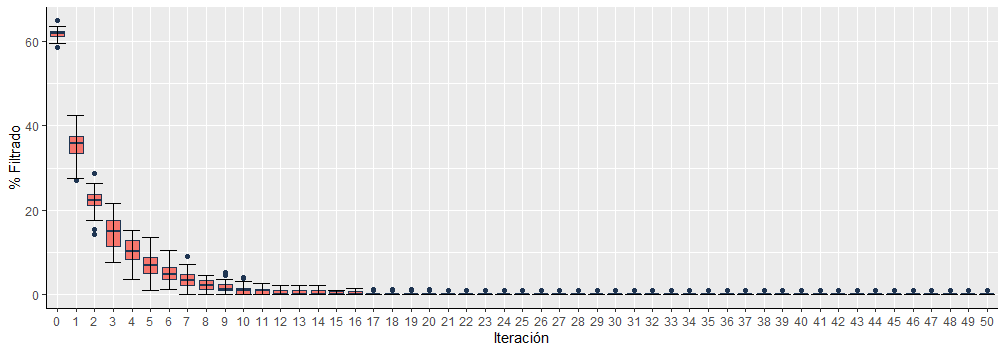
\includegraphics[width=170mm]{grafica1.png} % archivo
\end{figure}

\begin{figure} [h!]% figura
\renewcommand{\figurename}{Gráfica}
    \centering
    \caption{ K=200.}
    \label{grafica2}
    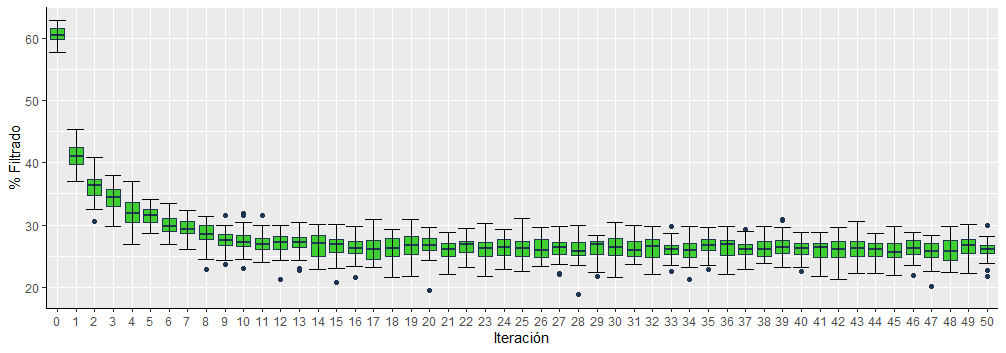
\includegraphics[width=170mm]{grafica2.png} % archivo
\end{figure}

\newpage
\begin{figure} [h!]% figura
\renewcommand{\figurename}{Gráfica}
    \centering
    \caption{ K=400.}
    \label{grafica3}
    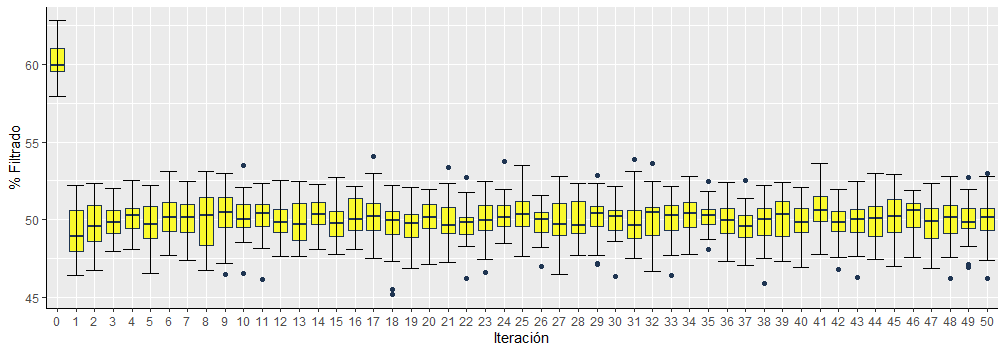
\includegraphics[width=170mm]{grafica3.png} % archivo
\end{figure}

\begin{lstlisting} [language=R, caption= Código para la obtención de las gráficas y pruebas estadísticas.]

png("p8_norm.png")
par(mfrow = c(2, 2)) # juntamos graficas
plot(density(originales)) # lo generado que era normal
print(shapiro.test(originales))
qqnorm(originales)
qqline(originales, col = 2)
plot(density(cumulos)) # lo nuestro que hemos modificado
print(shapiro.test(cumulos))
qqnorm(cumulos)
qqline(cumulos, col = 2)
graphics.off()

library(ggplot2)
datos$Iteracion = as.factor(datos$Iteracion)
datoss = split.data.frame(datos, f = datos$k)

ggplot(datoss$`100`, aes(x= Iteracion, y= filtrado)) + 
  geom_boxplot(fill = "#F8766D", colour = "#1F3552")+
  stat_boxplot(geom = "errorbar", width = 0.9)+
  theme(axis.line = element_line(colour = "black", size = 0.25))+
  labs(x = "Iteracion", y = "% Filtrado")

ggplot(datoss$`200`, aes(x= Iteracion, y= filtrado)) + 
  geom_boxplot(fill = "#3FCF30",colour = "#1F3552")+
  stat_boxplot(geom = "errorbar", width = 0.9)+
  theme(axis.line = element_line(colour = "black", size = 0.25))+
  labs(x = "Iteracion", y = "% Filtrado")

ggplot(datoss$`400`, aes(x= Iteracion, y= filtrado)) + 
  geom_boxplot(fill = "#FAFA2D",colour = "#1F3552")+
  stat_boxplot(geom = "errorbar", width = 0.9)+
  theme(axis.line = element_line(colour = "black", size = 0.25))+
  labs(x = "Iteracion", y = "% Filtrado")

library(tidyverse)
options(max.print=999999)

resul100<-datoss$`100`%>%
  group_by(Iteracion) %>%
  summarise(
    
    promedio = mean(filtrado, na.rm = TRUE),
    desviacion_std = sd(filtrado, na.rm = TRUE),
    varianza = sd(filtrado, na.rm = TRUE)^2,
    mediana = median(filtrado, na.rm = TRUE),
    rango_intercuartil = IQR(filtrado, na.rm = TRUE)
  )

resul200<-datoss$`200`%>%
  group_by(Iteracion) %>%
  summarise(
    
    promedio = mean(filtrado, na.rm = TRUE),
    desviacion_std = sd(filtrado, na.rm = TRUE),
    varianza = sd(filtrado, na.rm = TRUE)^2,
    mediana = median(filtrado, na.rm = TRUE),
    rango_intercuartil = IQR(filtrado, na.rm = TRUE)
  )


resul400<-datoss$`400`%>%
  group_by(Iteracion) %>%
  summarise(
    
    promedio = mean(filtrado, na.rm = TRUE),
    desviacion_std = sd(filtrado, na.rm = TRUE),
    varianza = sd(filtrado, na.rm = TRUE)^2,
    mediana = median(filtrado, na.rm = TRUE),
    rango_intercuartil = IQR(filtrado, na.rm = TRUE)
  )

shapiro100<-tapply(datoss$`100`$filtrado, datoss$`100`$Iteracion, shapiro.test)
shapiro200<-tapply(datoss$`200`$filtrado, datoss$`200`$Iteracion, shapiro.test)
shapiro400<-tapply(datoss$`400`$filtrado, datoss$`400`$Iteracion, shapiro.test)

one.way1<-aov(filtrado~Iteracion, data=datoss$`100`)
one.way11<-summary(one.way1)

one.way2<-aov(filtrado~Iteracion, data=datoss$`200`)
one.way22<-summary(one.way2)

one.way4<-aov(filtrado~Iteracion, data=datoss$`400`)
one.way44<-summary(one.way4)

one.wayt<-aov(filtrado~Iteracion, data=datos)
one.waytt<-summary(one.wayt)

pw100<-pairwise.wilcox.test(datoss$`100`$filtrado, datoss$`100`$Iteracion)

pw200<-pairwise.wilcox.test(datoss$`200`$filtrado, datoss$`200`$Iteracion)

pw400<-pairwise.wilcox.test(datoss$`400`$filtrado, datoss$`400`$Iteracion)

\end{lstlisting}

De las gráficas \ref{grafica1}, \ref{grafica2} y \ref{grafica3} podemos observar como aumenta el \% de filtrados conforme aumenta la k. Para poder observar la normalidad se realizaron las pruebas de Shapiro  Wilk \cite{shapiro} y ANOVA \cite{anova} además de que con la prueba Wilcox \cite{pairwise} se pueden apreciar las diferencias entre grupos, pese a que no es una prueba óptima se obtuvieron resultados favorables.

\begin{figure} [h!]% figura
\renewcommand{\figurename}{Gráfica}
    \centering
    \caption{ Ejemplo de estado inicial.}
    \label{grafica4}
    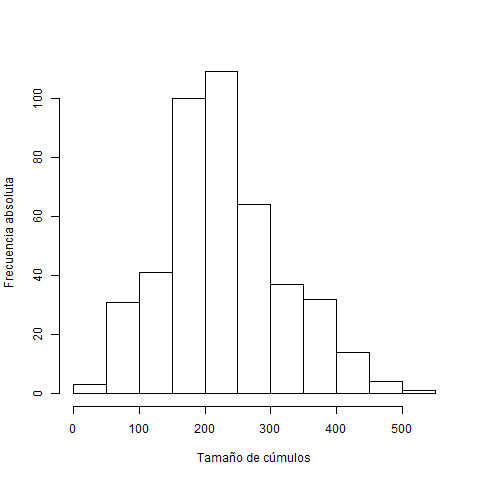
\includegraphics[width=100mm]{grafica4.png} % archivo
\end{figure}

\begin{figure} [h!]% figura
\renewcommand{\figurename}{Gráfica}
    \centering
    \caption{ Gráficas con distribución normal.}
    \label{grafica5}
    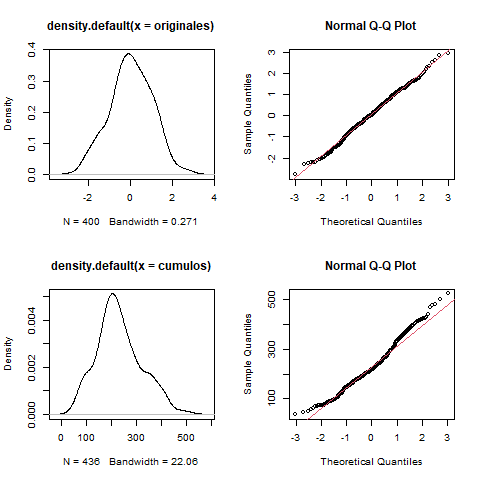
\includegraphics[width=100mm]{grafica5.png} % archivo
\end{figure}

\newpage

\begin{table}[h!]
\centering
\caption{Ejemplo de datos estadísticos obtenidos para k=100.}
\label{tabla2}
\begin{tabular}{|l|r|r|r|r|r|}
\hline
\multicolumn{1}{|c|}{\textbf{Iteración}} & \multicolumn{1}{c|}{\textbf{promedio}} & \multicolumn{1}{c|}{\textbf{desviación std}} & \multicolumn{1}{c|}{\textbf{varianza}} & \multicolumn{1}{c|}{\textbf{mediana}} & \multicolumn{1}{c|}{\textbf{rango intercuartil}} \\ \hline
0 & 61.71523 & 1.251743 & 1.566861 & 61.854 & 1.31775 \\ \hline
1 & 35.353 & 3.684828 & 13.57796 & 35.851 & 4.10225 \\ \hline
2 & 22.0904 & 3.343907 & 11.18171 & 22.3465 & 2.72025 \\ \hline
3 & 14.70127 & 3.729616 & 13.91003 & 15.054 & 6.0525 \\ \hline
4 & 10.40123 & 2.897143 & 8.393438 & 10.1935 & 4.546 \\ \hline
5 & 7.3204 & 3.168591 & 10.03997 & 7.007 & 3.78525 \\ \hline
6 & 5.127867 & 2.400151 & 5.760723 & 4.746 & 2.81 \\ \hline
7 & 3.519367 & 2.215608 & 4.90892 & 3.4655 & 2.57625 \\ \hline
8 & 2.3015 & 1.470262 & 2.161672 & 2.2485 & 2.293 \\ \hline
\end{tabular}
\end{table}

\begin{table}[h!]
\centering
\caption{Ejemplo de datos estadísticos obtenidos para k=200.}
\label{tabla3}
\begin{tabular}{|l|l|l|l|l|l|}
\hline
\multicolumn{1}{|c|}{\textbf{Iteración}} & \multicolumn{1}{c|}{\textbf{promedio}} & \multicolumn{1}{c|}{\textbf{desviación std}} & \multicolumn{1}{c|}{\textbf{varianza}} & \multicolumn{1}{c|}{\textbf{mediana}} & \multicolumn{1}{c|}{\textbf{rango intercuartil}} \\ \hline
0 & 60.57787 & 1.238704 & 1.534388 & 60.5265 & 1.74225 \\ \hline
1 & 41.02593 & 2.128901 & 4.53222 & 40.954 & 2.7095 \\ \hline
2 & 36.2149 & 2.390426 & 5.714138 & 36.376 & 2.5355 \\ \hline
3 & 34.29113 & 2.07091 & 4.288669 & 34.42 & 2.86925 \\ \hline
4 & 31.9951 & 2.275252 & 5.17677 & 31.847 & 3.14825 \\ \hline
5 & 31.4436 & 1.494179 & 2.232571 & 31.5385 & 2.085 \\ \hline
6 & 29.99557 & 1.404691 & 1.973156 & 29.815 & 2.13825 \\ \hline
7 & 29.35143 & 1.578227 & 2.490799 & 29.3635 & 1.84925 \\ \hline
8 & 28.45743 & 2.058751 & 4.238456 & 28.5345 & 2.3135 \\ \hline
\end{tabular}
\end{table}

\begin{table}[h!]
\centering
\caption{Ejemplo de datos estadísticos obtenidos para k=400.}
\label{tabla4}
\begin{tabular}{|l|r|r|r|r|r|}
\hline
\multicolumn{1}{|c|}{\textbf{Iteración}} & \multicolumn{1}{c|}{\textbf{promedio}} & \multicolumn{1}{c|}{\textbf{desviación std}} & \multicolumn{1}{c|}{\textbf{varianza}} & \multicolumn{1}{c|}{\textbf{mediana}} & \multicolumn{1}{c|}{\textbf{rango intercuartil}} \\ \hline
0 & 60.22247 & 1.198264 & 1.435837 & 59.9465 & 1.45875 \\ \hline
1 & 49.2111 & 1.612989 & 2.601732 & 48.9445 & 2.6865 \\ \hline
2 & 49.62313 & 1.494653 & 2.233989 & 49.5585 & 2.266 \\ \hline
3 & 49.93227 & 1.126089 & 1.268076 & 49.821 & 1.471 \\ \hline
4 & 50.18423 & 1.146516 & 1.314499 & 50.2575 & 1.30675 \\ \hline
5 & 49.75323 & 1.336128 & 1.785238 & 49.721 & 2.08425 \\ \hline
6 & 50.10557 & 1.222426 & 1.494326 & 50.167 & 1.85475 \\ \hline
7 & 50.08103 & 1.172139 & 1.373911 & 50.1475 & 1.81075 \\ \hline
8 & 49.96683 & 1.789549 & 3.202485 & 50.2665 & 3.034 \\ \hline
\end{tabular}
\end{table}

\newpage

\begin{table}[h!]
\centering
\caption{Ejemplo de resultados de la prueba Shapiro–Wilk para k=100.}
\label{tabla5}
\begin{tabular}{|l|r|r|}
\hline
\multicolumn{1}{|c|}{Iteración} & \multicolumn{1}{c|}{W} & \multicolumn{1}{c|}{P} \\ \hline
0 & 0.96596 & 0.4354 \\ \hline
1 & 0.97459 & 0.6705 \\ \hline
2 & 0.96884 & 0.508 \\ \hline
3 & 0.95827 & 0.2797 \\ \hline
4 & 0.97573 & 0.7042 \\ \hline
5 & 0.97921 & 0.8043 \\ \hline
6 & 0.95772 & 0.2706 \\ \hline
7 & 0.96945 & 0.5242 \\ \hline
8 & 0.93848 & 0.08279 \\ \hline
\end{tabular}
\end{table}

\begin{table}[h!]
\centering
\caption{Ejemplo de resultados de la prueba Shapiro–Wilk para k=200.}
\label{tabla6}
\begin{tabular}{|l|l|l|}
\hline
\multicolumn{1}{|c|}{Iteración} & \multicolumn{1}{c|}{W} & \multicolumn{1}{c|}{P} \\ \hline
0 & 0.98141 & 0.8617 \\ \hline
1 & 0.9849 & 0.9355 \\ \hline
2 & 0.98351 & 0.9092 \\ \hline
3 & 0.96734 & 0.4692 \\ \hline
4 & 0.99127 & 0.996 \\ \hline
5 & 0.96747 & 0.4724 \\ \hline
6 & 0.9745 & 0.6681 \\ \hline
7 & 0.97553 & 0.6983 \\ \hline
8 & 0.9473 & 0.1431 \\ \hline
\end{tabular}
\end{table}

\begin{table}[h!]
\centering
\caption{Ejemplo de resultados de la prueba Shapiro–Wilk para k=400.}
\label{tabla7}
\begin{tabular}{|l|l|l|}
\hline
\multicolumn{1}{|c|}{Iteración} & \multicolumn{1}{c|}{W} & \multicolumn{1}{c|}{P} \\ \hline
0 & 0.97893 & 0.7965 \\ \hline
1 & 0.96796 & 0.485 \\ \hline
2 & 0.97755 & 0.7572 \\ \hline
3 & 0.9688 & 0.5068 \\ \hline
4 & 0.9697 & 0.531 \\ \hline
5 & 0.97967 & 0.8167 \\ \hline
6 & 0.98276 & 0.8931 \\ \hline
7 & 0.96719 & 0.4655 \\ \hline
8 & 0.9572 & 0.2622 \\ \hline
\end{tabular}
\end{table}

\begin{table}[h!]
\centering
\caption{Resultados de la prueba ANOVA para varios valores de k.}
\label{tabla8}
\begin{tabular}{|c|r|r|r|r|r|}
\hline
k & \multicolumn{1}{c|}{\textbf{Df}} & \multicolumn{1}{c|}{\textbf{Sum Sq}} & \multicolumn{1}{c|}{\textbf{Mean Sq}} & \multicolumn{1}{c|}{\textbf{F value}} & \multicolumn{1}{c|}{\textbf{Pr(\textgreater{}F)}} \\ \hline
100 & 50 & 161461.06 & 3229.2212 & 2008.46572 & 0 \\ \hline
 & 1479 & 2377.94358 & 1.60780499 &  &  \\ \hline
200 & 50 & 44928.0908 & 898.561817 & 271.417384 & 0 \\ \hline
 & 1479 & 4896.41787 & 3.31062736 &  &  \\ \hline
400 & 50 & 3174.70437 & 63.4940873 & 36.2600481 & $1.148\times 10^{-218}$ \\ \hline
 & 1479 & 2589.84089 & 1.75107565 &  &  \\ \hline
Todos & 50 & 143653.377 & 2873.06753 & 7.44500087 & $1.9434\times 10^{-48}$ \\ \hline
 & 4539 & 1751625.52 & 385.905601 &  &  \\ \hline
\end{tabular}
\end{table}

\newpage

\begin{table}[h!]
\centering
\caption{Resultados de la prueba por parejas de Wilcox para k=100.}
\label{tabla9}
\begin{tabular}{|c|r|r|r|r|c|c|c|c|}
\hline
Iteración & \multicolumn{1}{c|}{\textbf{0}} & \multicolumn{1}{c|}{\textbf{1}} & \multicolumn{1}{c|}{\textbf{2}} & \multicolumn{1}{c|}{\textbf{3}} & \textbf{4} & 5 & 6 & 7 \\ \hline
1 & $2.2\times 10^{-14}$ & \multicolumn{1}{c|}{-} & \multicolumn{1}{c|}{-} & \multicolumn{1}{c|}{-} & - & - & - & - \\ \hline
2 & $2.2\times 10^{-14}$ & $2.6\times 10^{-13}$ & \multicolumn{1}{c|}{-} & \multicolumn{1}{c|}{-} & - & - & - & - \\ \hline
3 & $2.2\times 10^{-14}$ & $2.2\times 10^{-14}$ & $1.4\times 10^{-7}$ & \multicolumn{1}{c|}{-} & - & - & - & - \\ \hline
4 & $2.2\times 10^{-14}$ & $2.2\times 10^{-14}$ & $1.5\times 10^{-13}$ & 0.01169 & - & - & - & - \\ \hline
5 & $2.2\times 10^{-14}$ & $2.2\times 10^{-14}$ & $2.2\times 10^{-14}$ & $5.6\times 10^{-8}$ & \multicolumn{1}{r|}{0.2323} & - & - & - \\ \hline
6 & $2.9\times 10^{-8}$ & $2.9\times 10^{-8}$ & $2.9\times 10^{-8}$ & $7.8\times 10^{-8}$ & \multicolumn{1}{r|}{$2.4\times 10^{-5}$} & \multicolumn{1}{r|}{1} & - & - \\ \hline
7 & $2.9\times 10^{-8}$ & $2.9\times 10^{-8}$ & $2.9\times 10^{-8}$ & $3.6\times 10^{-8}$ & \multicolumn{1}{r|}{$3.7\times 10^{-7}$} & \multicolumn{1}{r|}{0.0094} & \multicolumn{1}{r|}{1} & - \\ \hline
8 & $2.9\times 10^{-8}$ & $2.9\times 10^{-8}$ & $2.9\times 10^{-8}$ & $2.9\times 10^{-8}$ & \multicolumn{1}{r|}{$5.8\times 10^{-8}$} & \multicolumn{1}{r|}{$9.3\times 10^{-6}$} & \multicolumn{1}{r|}{0.00297} & \multicolumn{1}{r|}{1} \\ \hline
\end{tabular}
\end{table}

\begin{table}[h!]
\centering
\caption{Resultados de la prueba por parejas de Wilcox para k=200.}
\label{tabla10}
\begin{tabular}{|c|l|l|l|l|c|c|c|c|}
\hline
Iteración & \multicolumn{1}{c|}{\textbf{0}} & \multicolumn{1}{c|}{\textbf{1}} & \multicolumn{1}{c|}{\textbf{2}} & \multicolumn{1}{c|}{\textbf{3}} & \textbf{4} & 5 & 6 & 7 \\ \hline
1 & $2.2\times 10^{-14}$ & \multicolumn{1}{c|}{-} & \multicolumn{1}{c|}{-} & \multicolumn{1}{c|}{-} & - & - & - & - \\ \hline
2 & $2.2\times 10^{-14}$ & $6.6\times 10^{-8}$ & \multicolumn{1}{c|}{-} & \multicolumn{1}{c|}{-} & - & - & - & - \\ \hline
3 & $2.2\times 10^{-14}$ & $2.2\times 10^{-13}$ & \multicolumn{1}{r|}{1} & \multicolumn{1}{c|}{-} & - & - & - & - \\ \hline
4 & $2.2\times 10^{-14}$ & $3.8\times 10^{-14}$ & $6.2\times 10^{-6}$ & \multicolumn{1}{r|}{0.12635} & - & - & - & - \\ \hline
5 & $2.2\times 10^{-14}$ & $2.2\times 10^{-14}$ & $3.6\times 10^{-9}$ & \multicolumn{1}{r|}{0.00035} & \multicolumn{1}{r|}{1} & - & - & - \\ \hline
6 & $2.2\times 10^{-14}$ & $2.2\times 10^{-14}$ & $6.7\times 10^{-12}$ & $9\times 10^{-9}$ & \multicolumn{1}{r|}{0.09026} & \multicolumn{1}{r|}{0.32849} & - & - \\ \hline
7 & $2.2\times 10^{-14}$ & $2.2\times 10^{-14}$ & $1.2\times 10^{-12}$ & $6\times 10^{-10}$ & \multicolumn{1}{r|}{0.00314} & \multicolumn{1}{r|}{0.0044} & \multicolumn{1}{r|}{1} & - \\ \hline
8 & $2.2\times 10^{-14}$ & $2.2\times 10^{-14}$ & $5.5\times 10^{-13}$ & $2\times 10^{-7}$ & \multicolumn{1}{r|}{$2.9\times 10^{-5}$} & \multicolumn{1}{r|}{$2\times 10^{-5}$} & \multicolumn{1}{r|}{1} & \multicolumn{1}{r|}{1} \\ \hline
\end{tabular}
\end{table}

\begin{table}[h!]
\centering
\caption{Resultados de la prueba por parejas de Wilcox para k=400.}
\label{tabla11}
\begin{tabular}{|c|l|l|l|l|c|c|c|c|}
\hline
Iteración & \multicolumn{1}{c|}{\textbf{0}} & \multicolumn{1}{c|}{\textbf{1}} & \multicolumn{1}{c|}{\textbf{2}} & \multicolumn{1}{c|}{\textbf{3}} & \textbf{4} & 5 & 6 & 7 \\ \hline
1 & $2.2\times 10^{-14}$ & \multicolumn{1}{c|}{-} & \multicolumn{1}{c|}{-} & \multicolumn{1}{c|}{-} & - & - & - & - \\ \hline
2 & $2.2\times 10^{-14}$ & 1 & \multicolumn{1}{c|}{-} & \multicolumn{1}{c|}{-} & - & - & - & - \\ \hline
3 & $2.2\times 10^{-14}$ & 1 & 1 & \multicolumn{1}{c|}{-} & - & - & - & - \\ \hline
4 & $2.2\times 10^{-14}$ & 1 & 1 & 1 & - & - & - & - \\ \hline
5 & $2.2\times 10^{-14}$ & 1 & 1 & 1 & \multicolumn{1}{l|}{1} & - & - & - \\ \hline
6 & $3.7\times 10^{-8}$ & 1 & 1 & 1 & \multicolumn{1}{l|}{1} & \multicolumn{1}{l|}{1} & - & - \\ \hline
7 & $2.2\times 10^{-14}$ & 1 & 1 & 1 & \multicolumn{1}{l|}{1} & \multicolumn{1}{l|}{1} & \multicolumn{1}{l|}{1} & - \\ \hline
8 & $2.2\times 10^{-14}$ & 1 & 1 & 1 & \multicolumn{1}{l|}{1} & \multicolumn{1}{l|}{1} & \multicolumn{1}{l|}{1} & \multicolumn{1}{l|}{1} \\ \hline
\end{tabular}
\end{table}

Se cambió el tamaño crítico al mínimo con \texttt{min} y se obtubieron las gráficas \ref{grafica6}, \ref{grafica7} y \ref{tabla8}.

\begin{figure} [h!]% figura
\renewcommand{\figurename}{Gráfica}
    \centering
    \caption{ k=100 con c al mínimo.}
    \label{grafica6}
    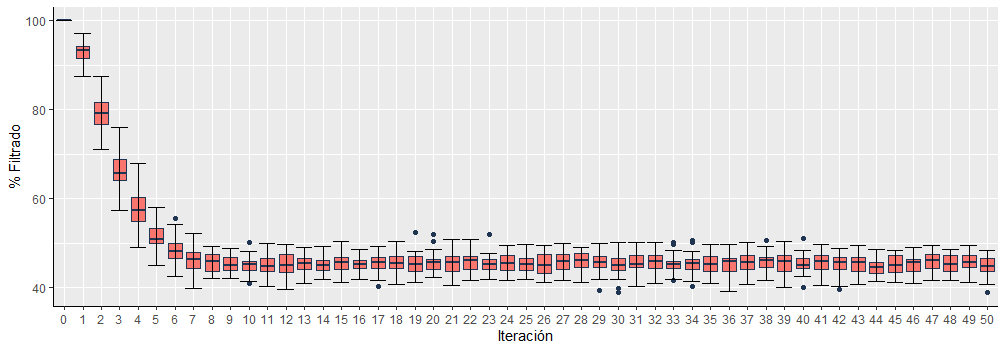
\includegraphics[width=170mm]{grafica6.png} % archivo
\end{figure}

\newpage

\begin{figure} [h!]% figura
\renewcommand{\figurename}{Gráfica}
    \centering
    \caption{ k=200 con c al mínimo.}
    \label{grafica7}
    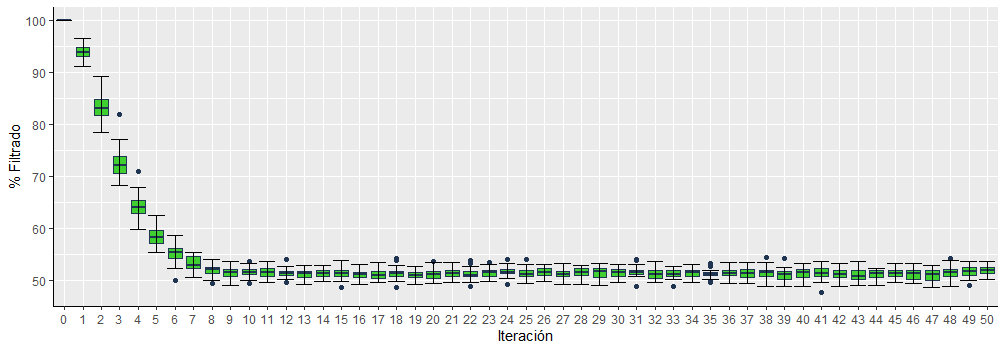
\includegraphics[width=170mm]{grafica7.png} % archivo
\end{figure}

\begin{figure} [h!]% figura
\renewcommand{\figurename}{Gráfica}
    \centering
    \caption{ k=400 con c al mínimo.}
    \label{grafica8}
    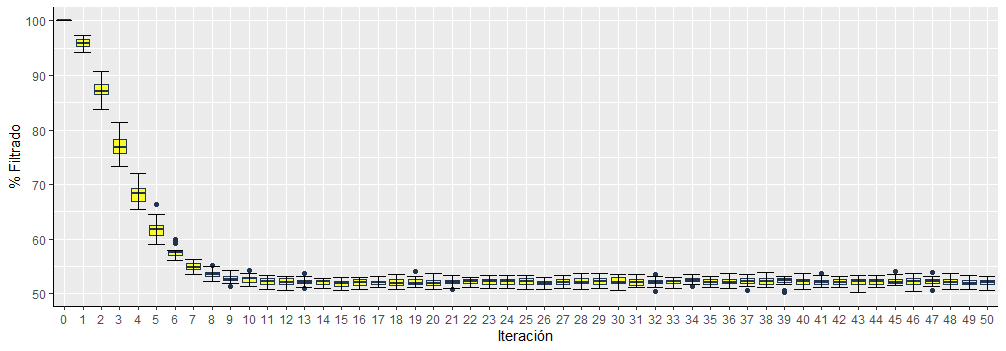
\includegraphics[width=170mm]{grafica8.png} % archivo
\end{figure}

\begin{lstlisting} [language=R, caption= Código para el cambio en el tamaño crítico.]

    assert(length(cumulos[cumulos == 0]) == 0) 
    assert(sum(cumulos) == n)
    c <- min(cumulos) 
    d <- sd(cumulos) / 4 

\end{lstlisting}

Del mismo modo se cambió el tamaño crítico al máximo con \texttt{max}.
\newpage

\begin{figure} [h!]% figura
\renewcommand{\figurename}{Gráfica}
    \centering
    \caption{ k=100 con c al máximo.}
    \label{grafica9}
    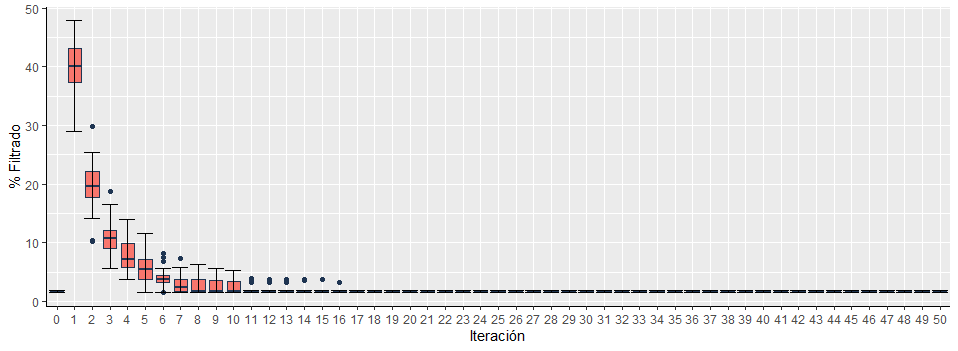
\includegraphics[width=170mm]{grafica9.png} % archivo
\end{figure}

\begin{figure} [h!]% figura
\renewcommand{\figurename}{Gráfica}
    \centering
    \caption{ k=200 con c al máximo.}
    \label{grafica10}
    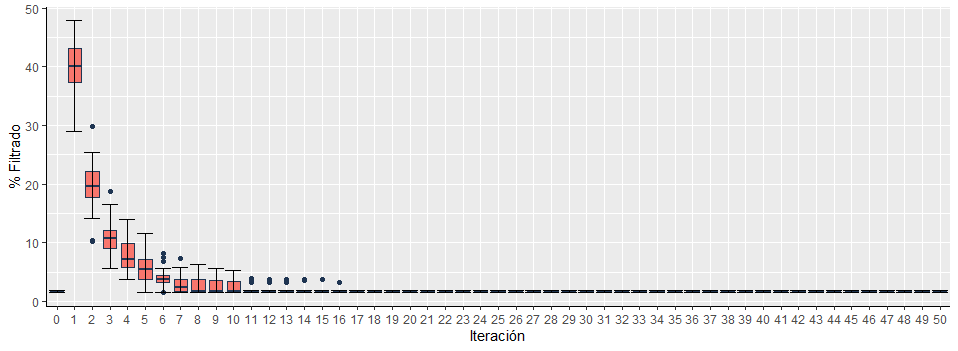
\includegraphics[width=170mm]{grafica10.png} % archivo
\end{figure}

\begin{figure} [h!]% figura
\renewcommand{\figurename}{Gráfica}
    \centering
    \caption{ k=400 con c al máximo.}
    \label{grafica11}
    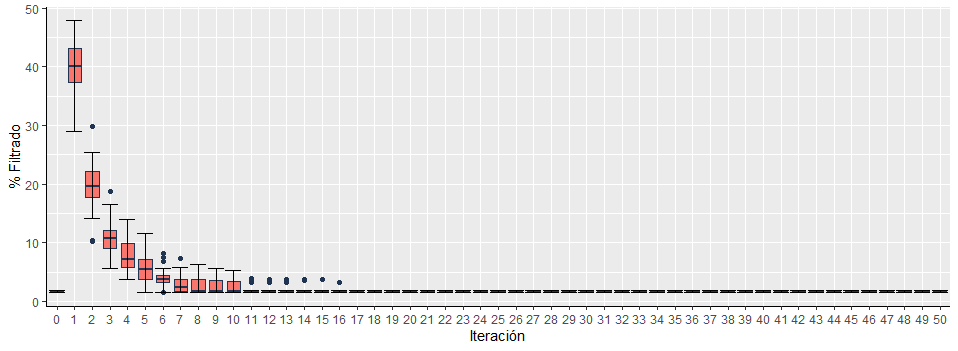
\includegraphics[width=170mm]{grafica11.png} % archivo
\end{figure}

\section{Conclusiones}
Con los resultados obtenidos podemos concluir que la k tiene una influencia en el porcentaje de filtración ya que este aumenta conforme lo hace la k hasta nivelarse alrededor del 50\% para la k grande y de las iteraciones la primera es la mejor filtración. De las pruebas de normalidad tenemos datos normales y de las de ANOVA se rechaza la hipótesis nula de que sus medias son iguales debido al elemento inicial que difiere bastante del resto de los elementos. En base a la prueba de wilcox se tiene una igualdad entre grupos a partir de la iteración 11 para k=100, la iteración 9 para k=200 y la iteración 1 para k=400, aunque no se considera una prueba fuerte para datos con distribución normal se obtuvieron interesantes resultados. De los cambios al tamaño crítico se pudo observar que con un tamaño mínimo filtraba todo al inicio y después se fue estabilizando hasta llegar al 50\% ya que con un tamaño crítico mínimo se forman menos cúmulos pero de mayor tamaño y así se logra filtrar más facilmente. Caso contrario al máximo donde al inicio no filtra nada ya que hay más cúmulos pero son mas pequeños.

\bibliography{referencias}
\bibliographystyle{plainnat}
\end{document}
